\documentclass{beamer}

\usepackage[utf8]{inputenc}
\usepackage{hyperref}

\usetheme{Berkeley}
\beamertemplatenavigationsymbolsempty
\setbeamertemplate{headline}{}
 
\title{Importing data into FoodChain-Lab 2}
\date{}
 
\begin{document}
\maketitle

\section{ }

\subsection{Tasks}
\begin{frame}
	\begin{itemize}
		\item In this part of the tutorial we will do a back- and forward-tracing from the "Frozen Fruit Sales" station.
		\item You can either complete part 1 of the tutorial or directly import the following files into an empty database before starting this tutorial.
		\item Start Template: \url{https://github.com/SiLeBAT/BfROpenLabResources/raw/master/GitHubPages/documents/Start_Tracing_Caterers.xlsx}
		\item Caterer 1 Template: \url{https://github.com/SiLeBAT/BfROpenLabResources/raw/master/GitHubPages/documents/Backtrace_request_Caterer 1.xlsx}
		\item Caterer 2 Template: \url{https://github.com/SiLeBAT/BfROpenLabResources/raw/master/GitHubPages/documents/Backtrace_request_Caterer 2.xlsx}
	\end{itemize}
\end{frame}
 
\subsection{1}
\begin{frame}
	\begin{center}
  		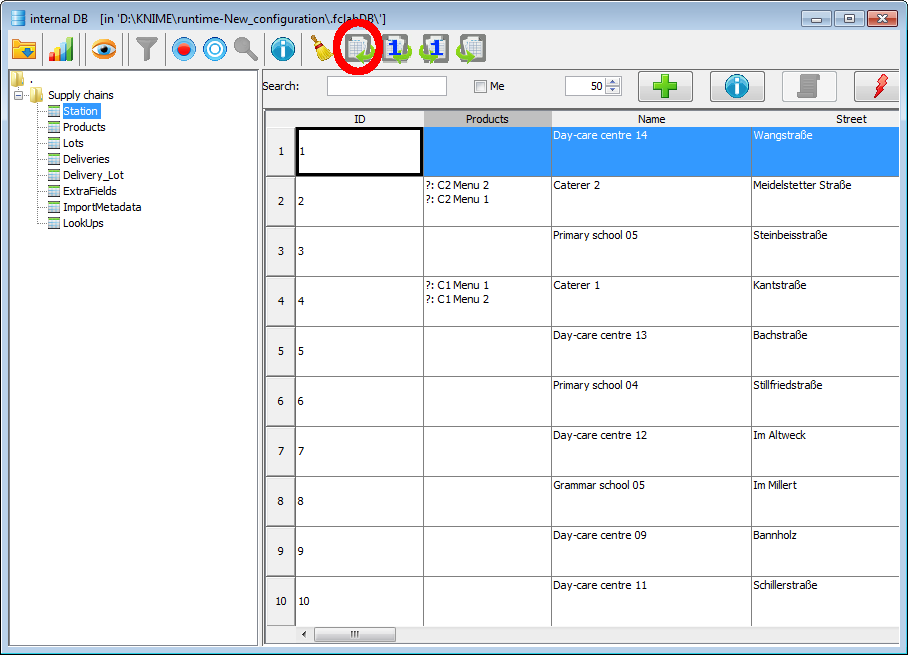
\includegraphics[height=0.6\textheight]{1.png}
	\end{center}
	\begin{itemize}
		\item You should have the database interface open.
		\item Press the button for generating backtracing templates, which is marked by the red circle.
	\end{itemize}
\end{frame}

\subsection{2}
\begin{frame}
	\begin{center}
  		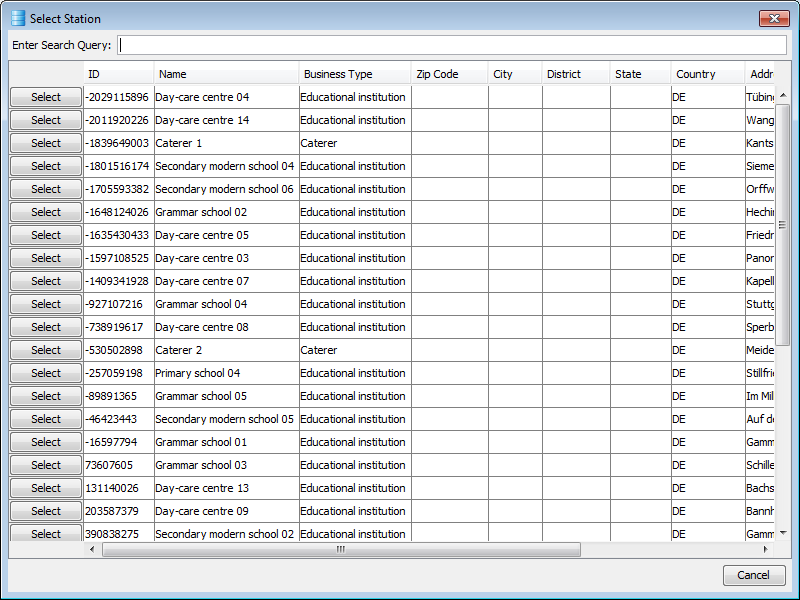
\includegraphics[width=0.4\textwidth]{2.png}
	\end{center}
	\begin{itemize}
		\item Since we want to do the backtracing for the supplier "Frozen Fruit Sales", select \textbf{Supplier} only and press \textbf{OK}.
	\end{itemize}
\end{frame}

\subsection{3}
\begin{frame}
	\begin{center}
  		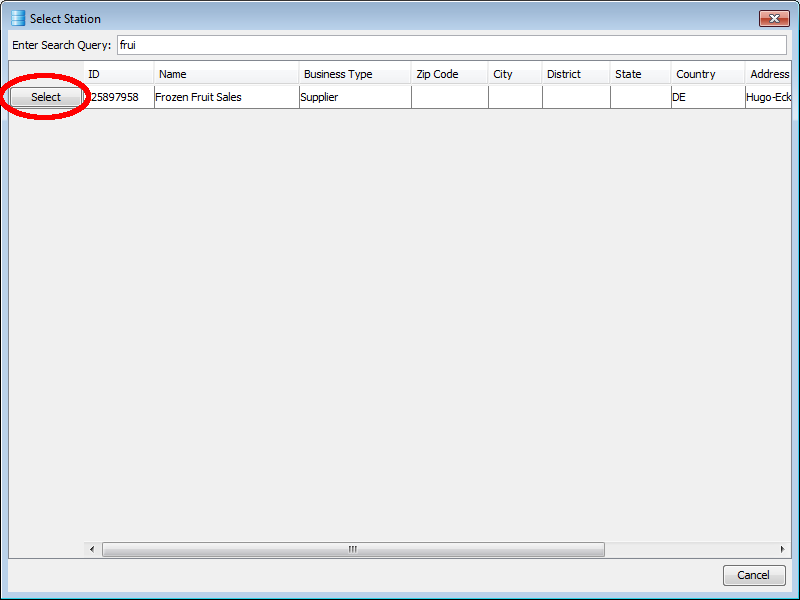
\includegraphics[height=0.5\textheight]{3.png}
	\end{center}
	\begin{itemize}
		\item In the file dialog that appears, you can specify the folder where the generated templates should be saved.
		\item Select the desired folder and press \textbf{Save}.
	\end{itemize}
\end{frame}

\subsection{4}
\begin{frame}
	\begin{center}
  		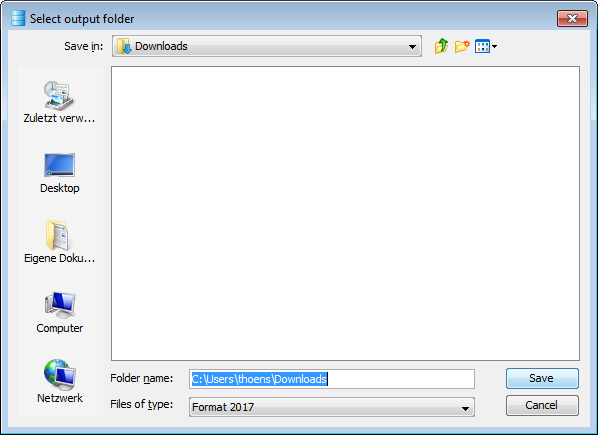
\includegraphics[width=0.8\textwidth]{4.png}
	\end{center}
	\begin{itemize}
		\item You'll be noticed, that one template was generated in the folder you specified.
		\item Press \textbf{OK}.
	\end{itemize}
\end{frame}

\subsection{5}
\begin{frame}
	\begin{center}
  		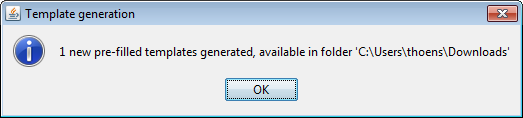
\includegraphics[width=0.95\textwidth]{5.png}
	\end{center}
	\begin{itemize}
		\item Open the generated template "Backtrace\_request\_Frozen Fruit Sales.xlsx".
		\item Add the stations from the screenshot to the \textbf{Stations} sheet.
		\item These station include 3 strawberry suppliers that delivered strawberries to "Frozen Fruit Sales" and also a caterer that received strawberries.
	\end{itemize}
\end{frame}

\subsection{6}
\begin{frame}
	\begin{center}
  		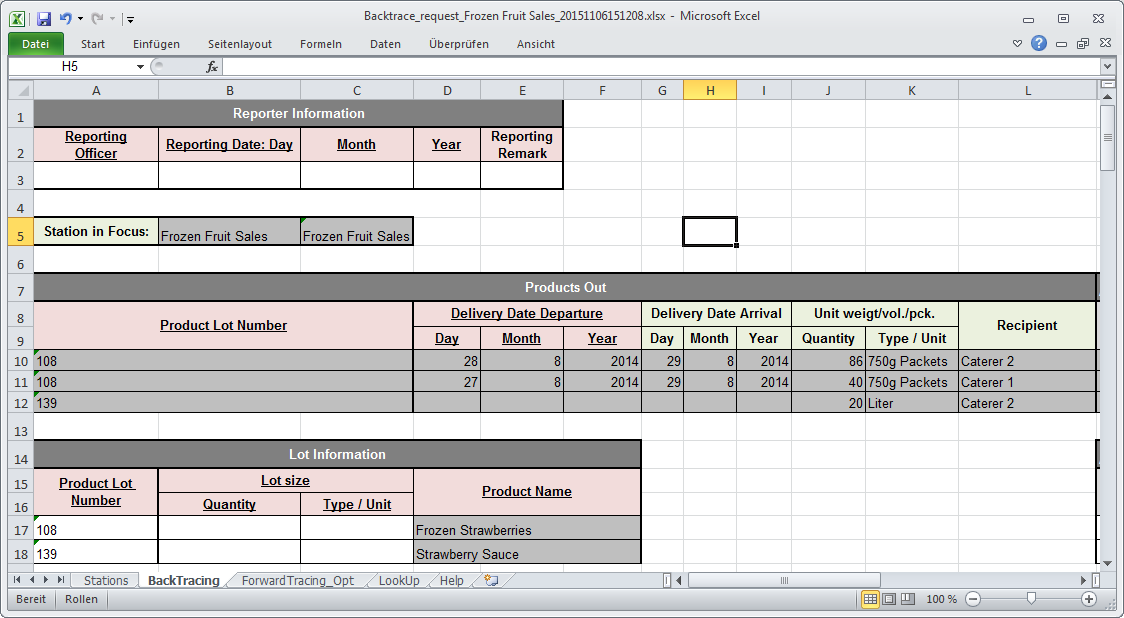
\includegraphics[width=0.95\textwidth]{6.png}
	\end{center}
	\begin{itemize}
		\item In the \textbf{BackTracing} sheet you can see the three outgoing deliveries of "Frozen Fruit Sales".
		\item These deliveries belong to lots "108" and "139".
	\end{itemize}
\end{frame}

\subsection{7}
\begin{frame}
	\begin{center}
  		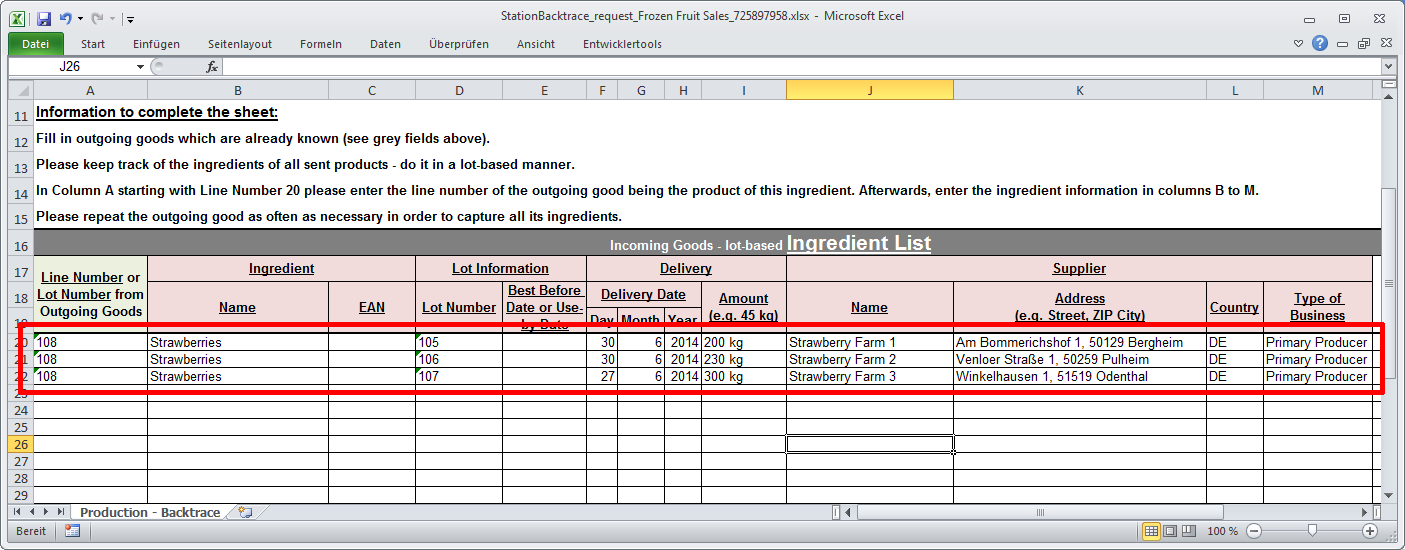
\includegraphics[width=0.95\textwidth]{7.png}
	\end{center}
	\begin{itemize}
		\item Now scroll to the \textbf{Ingredients for Lot(s)} section.
		\item Enter the 3 deliveries, that were used as ingredients for lot "108", from the screenshot.
	\end{itemize}
\end{frame}

\subsection{8}
\begin{frame}
	\begin{center}
  		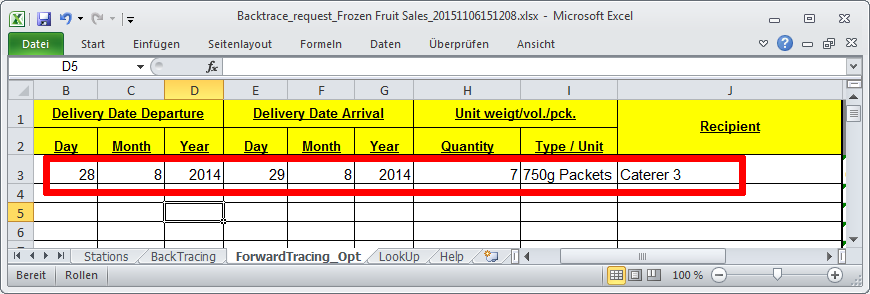
\includegraphics[width=0.95\textwidth]{8.png}
	\end{center}
	\begin{itemize}
		\item Lot "108" was not only delivered to "Caterer 1" and "Caterer 2", but also to a third caterer.
		\item We can add this information in the \textbf{ForwardTracing\_Opt} sheet.
		\item Enter the delivery to "Caterer 3" from the screenshot.
		\item Save the completed document ("Backtrace\_request\_Frozen Fruit Sales.xlsx").
	\end{itemize}
\end{frame}

\subsection{9}
\begin{frame}
	\begin{center}
  		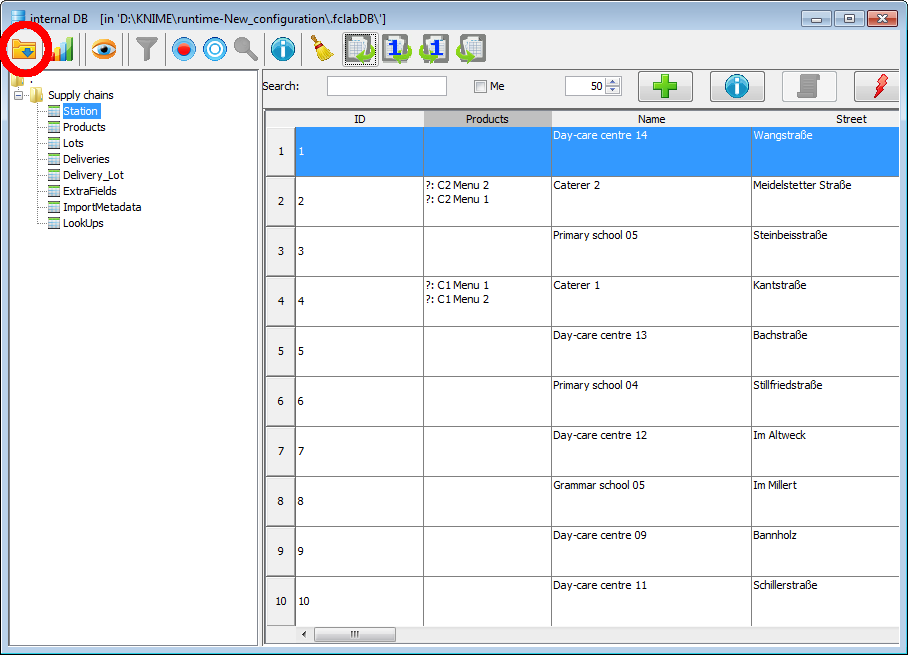
\includegraphics[height=0.6\textheight]{9.png}
	\end{center}
	\begin{itemize}
		\item To import this file click on the \textbf{Table import} button in the upper left corner of the database interface.
	\end{itemize}
\end{frame}

\subsection{10}
\begin{frame}
	\begin{center}
  		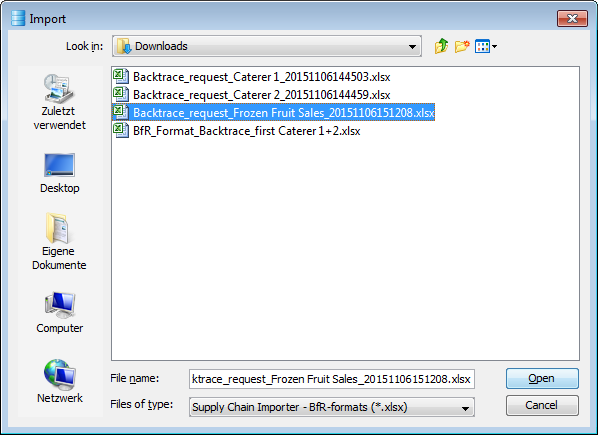
\includegraphics[height=0.5\textheight]{10.png}
	\end{center}
	\begin{itemize}
		\item In the file dialog that appears, select "Backtrace\_request\_Frozen Fruit Sales.xlsx" and press \textbf{Open}.
	\end{itemize}
\end{frame}

\subsection{11}
\begin{frame}
	\begin{center}
  		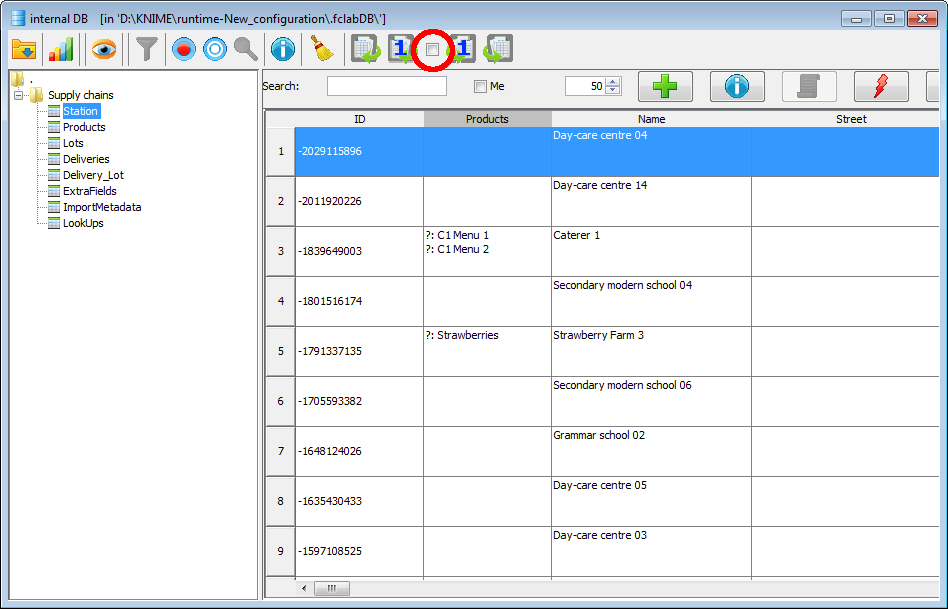
\includegraphics[width=0.7\textwidth]{11.png}
	\end{center}
	\begin{itemize}
		\item You'll be notified, that some warnings occurred during import.
		\item Press \textbf{Show Details} to have at look at the warnings.
	\end{itemize}
\end{frame}

\subsection{12}
\begin{frame}
	\begin{center}
  		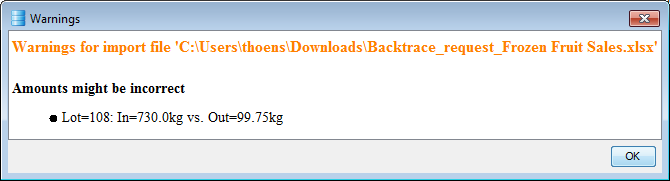
\includegraphics[width=0.95\textwidth]{12.png}
	\end{center}
	\begin{itemize}
		\item 730kg of strawberries went into lot "108", but all the deliveries of frozen strawberries from lot "108" just add up to 99.75kg.
		\item Warnings like these are supposed to help finding errors in the data.
		\item In this tutorial we just ignore the warning. So press \textbf{OK}.
	\end{itemize}
\end{frame}

\subsection{13}
\begin{frame}
	\begin{center}
  		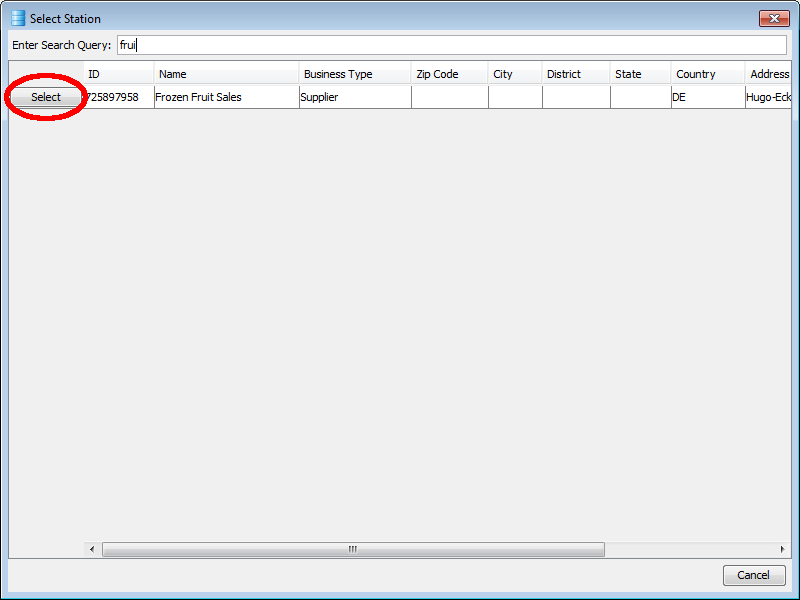
\includegraphics[height=0.6\textheight]{13.png}
	\end{center}
	\begin{itemize}
		\item We now know that lot "108" was also delivered to "Caterer 3" and we have imported this delivery into the database.
		\item Let's do a forward tracing from "Caterer 3".
		\item Press the button for generating the forward template for a specific station marked by the red circle.
	\end{itemize}
\end{frame}

\subsection{14}
\begin{frame}
	\begin{center}
  		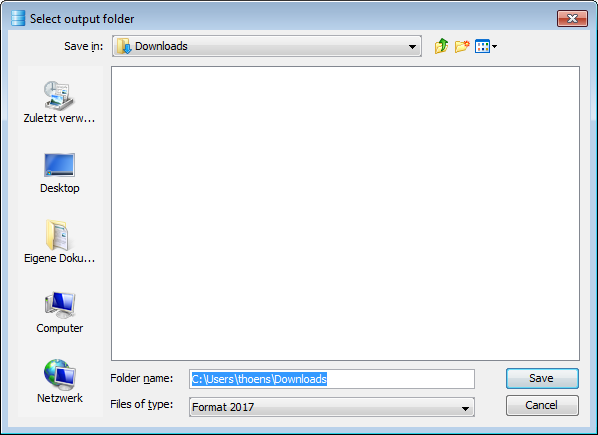
\includegraphics[width=0.95\textwidth]{14.png}
	\end{center}
	\begin{itemize}
		\item In the dialog that appears, you must select the station for which the template should be generated.
		\item Enter "cate" in the field after \textbf{Enter Search Query} and you will see that the table below only shows the caterers now.
		\item Press the \textbf{Select} button for "Caterer 3".
	\end{itemize}
\end{frame}

\subsection{15}
\begin{frame}
	\begin{center}
  		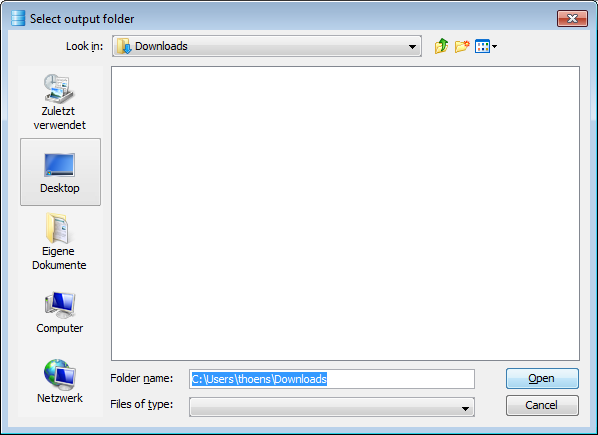
\includegraphics[height=0.5\textheight]{15.png}
	\end{center}
	\begin{itemize}
		\item In the file dialog that appears, you can specify the folder where the generated templates should be saved.
		\item Select the desired folder and press \textbf{Save}.
	\end{itemize}
\end{frame}

\subsection{16}
\begin{frame}
	\begin{center}
  		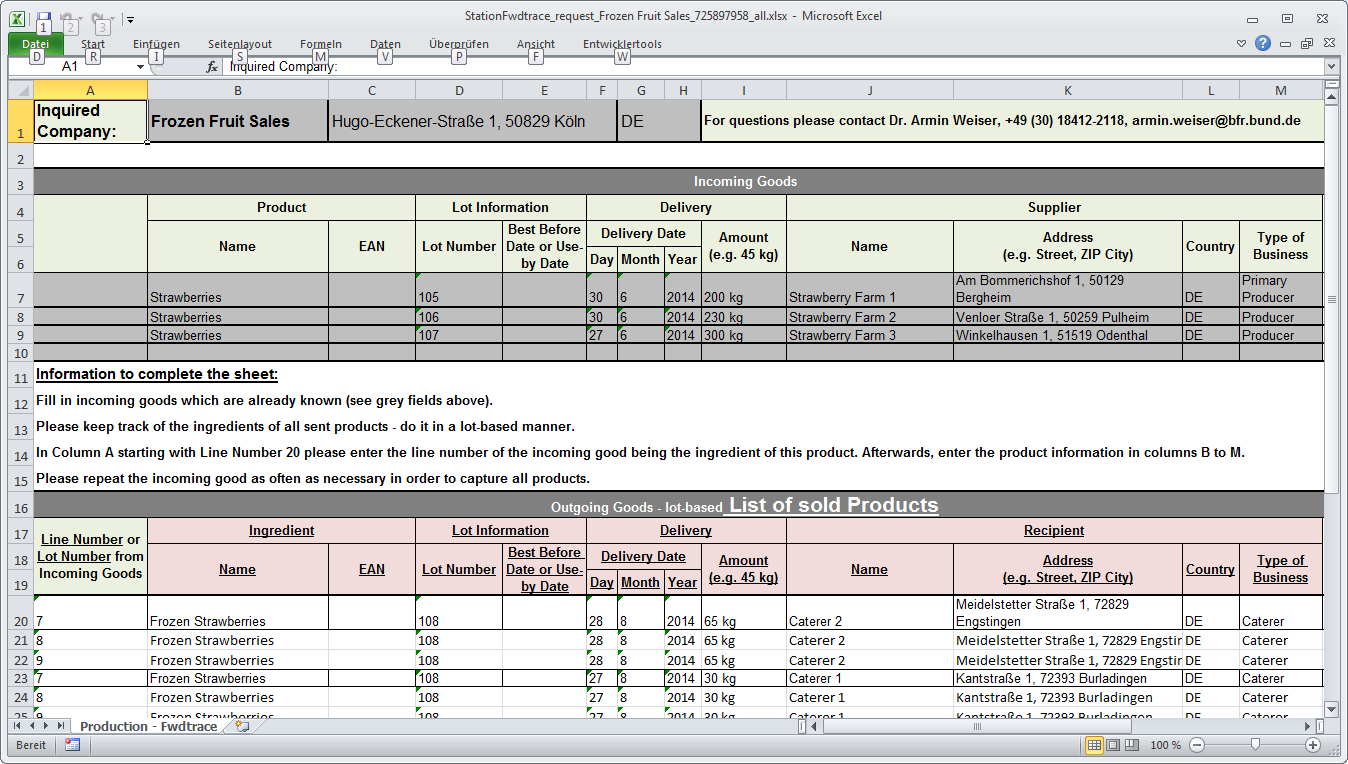
\includegraphics[width=0.8\textwidth]{16.png}
	\end{center}
	\begin{itemize}
		\item You'll be noticed, that one template was generated in the folder you specified.
		\item Press \textbf{OK}.
	\end{itemize}
\end{frame}

\subsection{17}
\begin{frame}
	\begin{center}
  		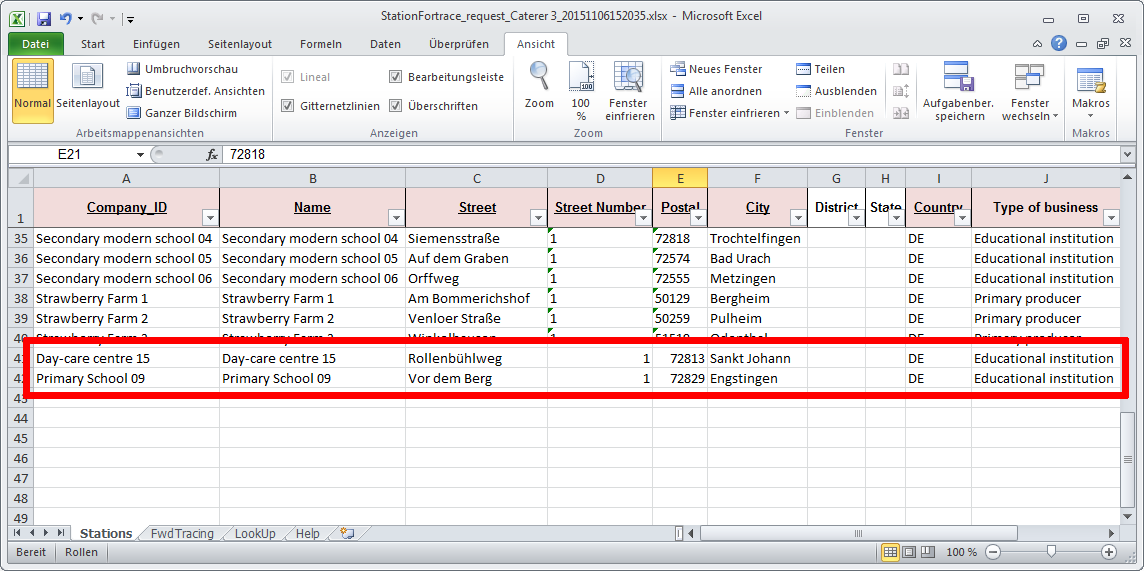
\includegraphics[width=0.95\textwidth]{17.png}
	\end{center}
	\begin{itemize}
		\item Open "StationFwdtrace\_request\_Caterer 3.xlsx".
		\item Enter the station from the screenshot in the \textbf{Stations} sheet.
	\end{itemize}
\end{frame}

\subsection{18}
\begin{frame}
	\begin{center}
  		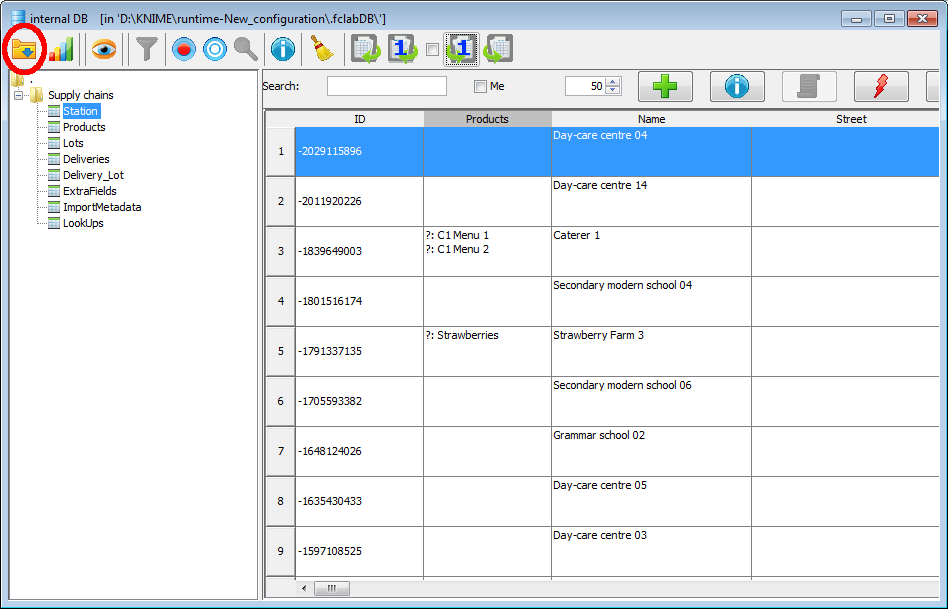
\includegraphics[width=0.9\textwidth]{18.png}
	\end{center}
	\begin{itemize}
		\item In the \textbf{FwdTracing} sheet you first have to enter all relevant outgoing lots of "Caterer 3". So add lot "C3M1" to the \textbf{Lot Information} section as shown on the screenshot (red rectangle).
		\item Now you can specify, that the delivery of "Frozen Strawberries" was used as an ingredient in this lot (red circle).
	\end{itemize}
\end{frame}

\subsection{19}
\begin{frame}
	\begin{center}
  		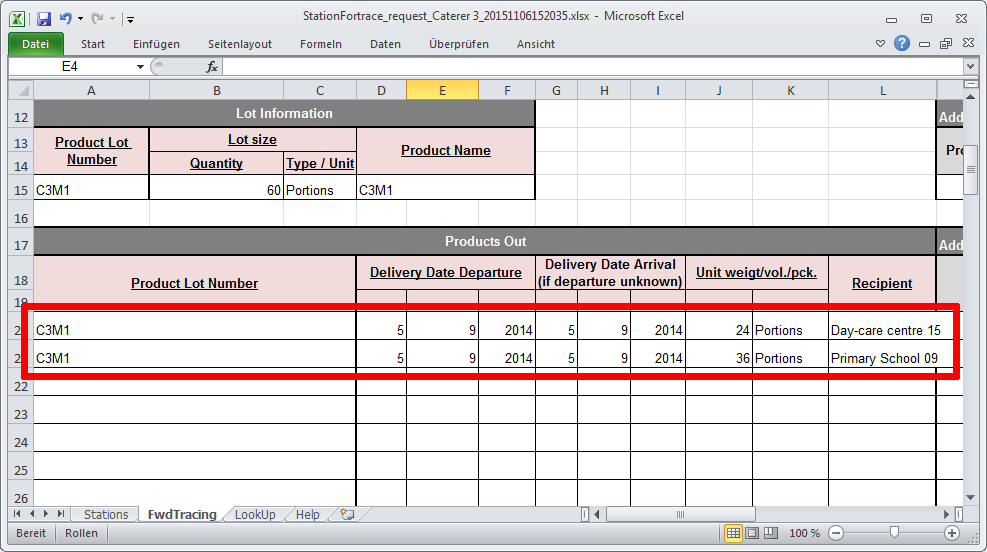
\includegraphics[width=0.95\textwidth]{19.png}
	\end{center}
	\begin{itemize}
		\item Scroll down to the \textbf{Products Out} section to specify the outgoing deliveries from lot "C3M1".
		\item Add the deliveries as shown on the screenshot.
		\item Save the completed document ("StationFwdtrace\_request\_Caterer 3.xlsx").
	\end{itemize}
\end{frame}

\subsection{20}
\begin{frame}
	\begin{center}
  		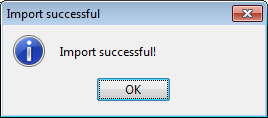
\includegraphics[height=0.6\textheight]{20.png}
	\end{center}
	\begin{itemize}
		\item To import this file click on the \textbf{Table import} button in the upper left corner of the database interface.
	\end{itemize}
\end{frame}

\subsection{21}
\begin{frame}
	\begin{center}
  		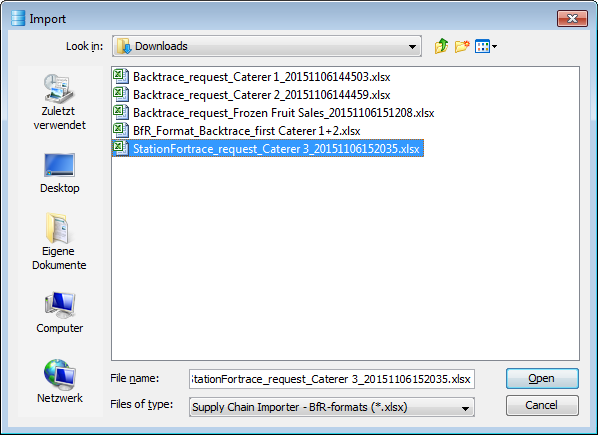
\includegraphics[height=0.5\textheight]{21.png}
	\end{center}
	\begin{itemize}
		\item In the file dialog that appears, select "StationFwdtrace\_request\_Caterer 3.xlsx" and press \textbf{Open}.
	\end{itemize}
\end{frame}

\subsection{22}
\begin{frame}
	\begin{center}
  		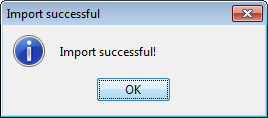
\includegraphics[width=0.4\textwidth]{22.png}
	\end{center}
	\begin{itemize}
		\item You'll see a message that the import was successful.
		\item Press \textbf{OK}.
	\end{itemize}
\end{frame}

\end{document}